\documentclass{article}

% Language setting
% Replace `english' with e.g. `spanish' to change the document language
\usepackage[english]{babel}

% Set page size and margins
% Replace `letterpaper' with `a4paper' for UK/EU standard size
\usepackage[letterpaper,top=2cm,bottom=2cm,left=3cm,right=3cm,marginparwidth=1.75cm]{geometry}

% Useful packages
\usepackage{amsmath}
\usepackage{amssymb}
\usepackage{mathtools}
\usepackage{graphicx}
\usepackage[colorlinks=true, allcolors=blue]{hyperref}
\usepackage{subcaption}
\usepackage[normalem]{ulem}
\usepackage[framemethod=TikZ]{mdframed}
\newtheorem{prop}{Proposition}
\newtheorem{lem}{Lemme}
\newtheorem{rem}{Remarque}
\newcounter{mydef}[section]\setcounter{mydef}{0}
\renewcommand{\themydef}{\arabic{section}.\arabic{mydef}}

\definecolor{newtext}{HTML}{c0edad}
\newenvironment{new}{\begin{mdframed}[linewidth=0pt,backgroundcolor=newtext]}{\end{mdframed}}

\newenvironment{definition}[2][]{%
    \refstepcounter{mydef}
 
    \ifstrempty{#1}%
    % if condition (without title)
    {\mdfsetup{%
        frametitle={%
            \tikz[baseline=(current bounding box.east),outer sep=0pt]
            \node[anchor=east,rectangle,fill=gray!20,rounded corners=3pt]
            {\strut Definition~\themydef};}
        }%
    % else condition (with title)
    }{\mdfsetup{%
        frametitle={%
            \tikz[baseline=(current bounding box.east),outer sep=0pt]
            \node[anchor=east,rectangle,fill=gray!20,rounded corners=3pt]
            {\strut Definition~\themydef:~#1};}%,
        }%
    }%
    % Both conditions
    \mdfsetup{%
        innertopmargin=10pt,linecolor=gray!20,%
        linewidth=2pt,topline=true,%
        frametitleaboveskip=\dimexpr-\ht\strutbox\relax,%
        roundcorner=5pt,
        nobreak=true
    }
\begin{mdframed}[]\relax}{%
\end{mdframed}}



\title{}
\author{Lysandre Macke}

\begin{document}
% \maketitle

\section{Definition}

\subsection{Rappel}
Dans un premier lieu, il est important de rappeler la notion de courbe $(\theta, \delta)$-CTLB.

\begin{definition}[Courbe $(\theta, \delta)$-CTLB]{}
Une courbe de Jordan $\mathcal{C}$ est dite $(\theta, \delta)$-CTLB si pour toute paire de point $a$, $b \in  \mathcal{C}$ tels que d$(a, b) < \delta$, on a $\mathcal{K}(\mathcal{C}_a^b) \leq \theta$.    
\end{definition}

Par la suite, nous appellerons courbe $\delta$-CTLB une courbe CTLB de paramètre $\theta = \frac{\pi}{2}$.

Nous donnons une définition d'une surface $\delta$-CTLB comme suit :

\begin{definition}[Surface $\delta$-CTLB]{}
Une surface $\mathcal{S}$ est dite $\delta$-CTLB si pour toute paire de points $a$, $b$ de $\mathcal{S}$ tels que d$(a, b) < \delta$ il existe au moins un arc $\mathcal{C}_a^b$ de courbure totale inférieure ou égale à $\frac{\pi}{2}$.
\end{definition}
\begin{new}

\subsection{Le cube comme surface \texorpdfstring{$\delta$}-CTLB}
Soit un cube $C$ de longueur $c$. Montrons que $C$ est $c$-CTLB. Autrement dit, on va chercher à montrer que pour \textbf{toute paire de points $A, B$ tels que $d(A, B) < c$ il existe au moins un arc $\mathcal{C}_a^b$ tel que  $\mathcal{k}(\mathcal{C}_a^b) \leq \frac{\pi}{2}$}. Toute paire de points $A$ et $B$ à distance strictement inférieure à $c$ sont soit sur une même face du cube, soit sur deux faces opposées. Dans le premier cas, il est possible de tracer le segment reliant $A$ et $B$, ce dernier ayant une courbure totale nulle. Dans le second cas, on pose $A'$ le projeté orthogonal de $A$ sur l'arête $a$ séparant les deux points. On a donc $AA'$ orthogonal à $A'B$, et la ligne polygonale $AA'B$ est de courbure totale $\frac{\pi}{2}$. Ainsi, un cube de longueur $c$ est $c$-CTLB.

\end{new}
%---------------------

\subsection{Al-Kashi}

\begin{figure}[!h]
    \centering
    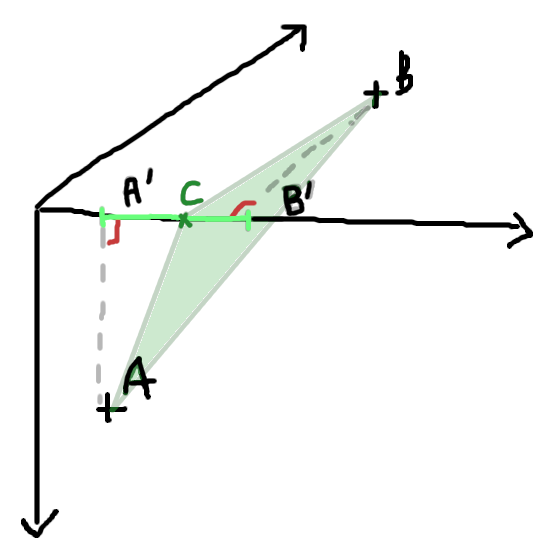
\includegraphics[width=0.3\linewidth]{al_kashi.png}
    \caption{Illustration des points}
    \label{fig:al_kashi}
\end{figure}

Soient $A(0, y_A, z_A)$ et $B(x_B, 0, z_B)$ deux points situés sur deux faces adjacentes du cube. Soit $C(0, 0, z_C)$ un point de l'arête séparant ces deux faces.\\
Notons $\theta := \kappa([A, C, B])$ la courbure de la ligne polygonale formée par $A$, $B$ et $C$.

Les points $A$ $B$ et $C$ forment un triangle, et par Al-Kashi on a : 
$$ AB^2 = AC^2 - 2 \cos(\pi - \theta)ACBC + BC^2 $$
% De plus, par pythagore on a : 
% $$BC^2 = BB'^2 + B'C^2 \quad \text{et} \quad AC^2 = AA'^2 + A'C^2$$
% En se servant de $A'B'= A'C + B'C$, on a donc,
% $$BC^2 = BB'^2 + (A'B' - A'C)^2 = BB'^2 + A'B'^2 - 2A'B' A'C + A'C^2$$

D'où :

\begin{align*}
    \cos(\pi - \theta) &= \frac{-AB^2 + AC^2 + BC^2}{2AC BC}\\
    &= \frac{-(z_A - z_B)^2 + (z_A - z_C)^2 + (z_B- z_C)^2}{2\sqrt{y_A^2 + (z_A - z_C)^2}\sqrt{x_B^2 + (z_B - z_C)^2}}
    %cos^2(\pi - \theta) &= \frac{(-AB^2 + AC^2 + BC^2)^2}{4AC^2 BC^2}\\
    %&= \frac{(-AB^2 +  AA'^2 + A'C^2 + BB'^2 + A'B'^2 - 2A'B' A'C + A'C^2)^2}{4(AA'^2 + A'C^2)(BB'^2 + A'B'^2 - 2A'B' A'C + A'C^2)}\\
    %&= \frac{(-d^2 +  H^2 + x^2 + l^2 - 2lx + x^2)^2}{4(AA'^2 + x^2)(BB'^2 + l^2 - 2lx + x^2)}\\
    %&= \frac{(-d^2 +  H^2 + 2x^2 + l^2 - 2lx)^2}{4(AA'^2 + x^2)(BB'^2 + l^2 - 2lx + x^2)}\\
    %&= \frac{(-d^2 +  H^2 + l^2 + 2x(-l + x))^2}{4(AA'^2 + x^2)(BB'^2 + l^2 - 2lx + x^2)}\\
\end{align*}

Notons $f$ cette fonction.\\
$f$ s'annule en $z_C = z_A$ et $z_c = z_B$, où on a alors $\pi - \theta = \arccos(0)$ et donc $\theta = \frac{\pi}{2}$.\\
Comme la fonction cosinus est continue par définition, et que $f$ ne s'annule pas sur $]z_A, z_B[$, on sait qu'elle est soit positive soit négative sur cet ensemble.\\
Le dénominateur était positif car produit de fonctions positives, on se restreint à l'étude de signe du numérateur $u(z_C) = -(z_A - z_B)^2 + (z_A - z_C)^2 + (z_B- z_C)^2$.\\
On a $u'(z_C) = 4z_C - 2z_A - 2z_B$ linéaire et croissante sur $\mathbb{R}$, $u$ est donc convexe sur $\mathbb{R}$ et donc sur $[z_A, z_B]$.\\
Ainsi, \underline{pour tout $z_C \in [z_A, z_B]$, $f(z_C) \leq 0$, et donc $\theta \leq \frac{\pi}{2}$}.

\subsubsection{recherche de minimum}
 En reprenant $f$ comme défini précédemment, on a : 
\begin{align*}
    f'(z_C) &= - \frac{z_A + z_B - 2z_C}{\sqrt{x_B^2 + (z_B - z_C)^2} \sqrt{y_A^2 + (z_A - z_C)^2}} \\
    &- \frac{(z_A - z_B)^2 - (z_A - z_C)^2 - (z_B - z_C)^2}{2\sqrt{x_B^2 + (z_B - z_C)^2} \cdot (y_A^2 + (z_A - z_C)^2)^{3/2}} \cdot (z_A - z_C) \\
    &- \frac{(z_A - z_B)^2 - (z_A - z_C)^2 - (z_B - z_C)^2}{2(x_B^2 + (z_B - z_C)^2)^{3/2} \cdot \sqrt{y_A^2 + (z_A - z_C)^2}} \cdot (z_B - z_C)
\end{align*}

La racine réelle de $f'$ est :
$$z_C = \frac{1}{3} \left( \frac{3 \left( x_B^2 z_A + y_A^2 z_B \right)^2}{\left( x_B^2 + y_A^2 \right)^2} - \frac{3 y_A^2 z_B^2 + \left( 2 y_A^2 + 3 z_A^2 \right) x_B^2}{x_B^2 + y_A^2} \right) \Bigg/ \left( \frac{1}{6} \sqrt{ \frac{32}{3} x_B^4 y_A^2 + \frac{32}{3} x_B^2 y_A^4 + 9 z_A^6 - 54 z_A z_B^5 + 9 z_B^6 + 18 \left( x_B^2 + y_A^2 \right) z_A^4 + 9 \left( 2 x_B^2 + 2 y_A^2 + 15 z_A^2 \right) z_B^4 - 36 \left( 5 z_A^3 + 2 \left( x_B^2 + y_A^2 \right) z_A \right) z_B^3 + 3 \left( 3 x_B^4 + 10 x_B^2 y_A^2 + 3 y_A^4 \right) z_A^2 + 3 \left( 3 x_B^4 + 10 x_B^2 y_A^2 + 3 y_A^4 + 45 z_A^4 + 36 \left( x_B^2 + y_A^2 \right) z_A^2 \right) z_B^2 - 6 \left( 9 z_A^5 + 12 \left( x_B^2 + y_A^2 \right) z_A^3 + \left( 3 x_B^4 + 10 x_B^2 y_A^2 + 3 y_A^4 \right) z_A \right) z_B } \frac{x_B^2 y_A^2}{\left( x_B^2 + y_A^2 \right)^2} + \frac{\left( x_B^2 z_A + y_A^2 z_B \right)^3}{\left( x_B^2 + y_A^2 \right)^3} - \frac{1}{2} \frac{3 y_A^2 z_B^2 + \left( 2 y_A^2 + 3 z_A^2 \right) x_B^2}{x_B^2 + y_A^2} \cdot \frac{ \left( x_B^2 z_A + y_A^2 z_B \right)}{\left( x_B^2 + y_A^2 \right)^2} + \frac{1}{2} \frac{y_A^2 z_B^3 + \left( y_A^2 \left( z_A + z_B \right) + z_A^3 \right) x_B^2}{x_B^2 + y_A^2} \right)^{\frac{1}{3}} + \frac{x_B^2 z_A + y_A^2 z_B}{x_B^2 + y_A^2}$$

\subsubsection{Le cube non $\delta$-CTLB pour $\delta > c$}

On veut montrer que le cube n'est pas $\delta$-CTLB pour $\delta > c$, autrement dit que pour tout $A$ et $B$ situés sur des faces opposées, toute ligne polygonale les reliant est de courbure totale strictement inférieure à $\frac{\pi}{2}$.\\
Soient $A$ et $B$ situés sur des faces opposées. On sait que la ligne polygonale entre $A$ et $B$ est nécessairement formée par au moins quatre points $A$, $B$, avec $C$ et $D$ situés sur deux arêtes parallèles séparant $A$ et $B$. Ainsi, l'angle entre $CD$ et l'une ou l'autre de ces arêtes est nécessairement borné par $[\frac{\pi}{4}, \frac{\pi}{2}]$.
% avec 
% \begin{align*}
%     d &= AB,\\
%     l &= A'B', \\
%     H^2 &= AA'^2 + BB'^2,\\
%     x &= A'C \in [0, l]
% \end{align*}
% En notant $z:= 2x(l-x) -H^2-l^2 \in [?, ?]$ (TO DO: déterminer les bornes)
% $$ cos^2 \theta = - \frac{(d^2-z)^2}{z} $$ 

% que l'on cherche à maximiser (pour minimiser $\theta$ si $cos \theta \geq 0$) et à minimiser (pour minimiser $\theta$ si $cos \theta \leq 0$).
% 2 possibilités: soit l'extremum $z_{extremum}$ trouvé en $z$ est atteignable par $z(x)$, on fait le changement de variable inverse pour retrouver  $x$, sinon on essaie le $x$ qui minimise $z(x) -z_{extremum}$. 

\subsection{Preuve géométrique}

%On s’intéresse au cas où on a un point sur une face d’un cube et un autre sur une face adjacente. On cherche à montrer qu’il existe un chemin entre ces deux points dont l’angle est inférieur ou égal à pi/2. 
Dans toute la suite, angle désigne l’angle externe. on suppose qu'aucun des deux point A, B n'appartient à l'arête

%\begin{prop}
%si on déplie les deux faces de sorte à ce qu’elles soient dans le même plan, alors le segment de droite qui relie les deux points croise l’arête en un point qui donne un angle minimal sur le cube.
%\end{prop}
%Preuve : 
Soit $A^r$ le point $A$ déplié. Pour tout point P de l’arête, la longueur de APB est égale à celle d’$A^rPB$ car elle est la somme de la longueur des segments $A^rP$ et $PB$ qui est invariante par la rotation (d’axe l’arête) transformant $A$ en $A^r$. Or la longueur d’$A^rCB$ est plus petite que celle d’$A^rC’B$ par définition~: elle est minimale et il en va donc de même pour $ACB.$


%\begin{lem}
%Soit A et B deux points de $\mathbb{R}^3$ et deux points P et P’ distincts de A et B tels que $|AP|<|AP’|$ et $|BP|<|BP’|$ alors les angles $APB<AP’B$.
%\end{lem}
%Preuve : on peut, en appliquant un rotation d’axe (AB) ramener point P’ dans le plan APB de sorte à ce que le triangle APB soit contenu dans le triangle AP’B. C’est une transformation rigide qui ne modifie pas les angles du triangle AP’B. De cette inclusion, on déduit que l’angle APB est strictement inférieur à l’angle AP’B.  

%Les point C et C’ respectent les hypothèses du lemme par rapport à A et B. Ainsi l’angle ACB est minimal. 

On note $A^\perp$ est le projeté orthogonal de $A$ sur l’arête, et de même pour $B$.
\begin{lem}
Les angles  $AA^\perp B$ et $AB^\perp B$ sont droits.
\end{lem}
En effet, $A^\perp$ est le projeté orthogonal sur l’arête, le segment $AA^\perp$ est orthogonal à la face contenant B et donc à B lui-même. 

Ainsi ACB est inférieur ou égal à $AA^\perp B=\pi/2$ et le cas d’égalité est pour $A^\perp =B^\perp $

\begin{rem}
On obtient 
\begin{itemize}
    \item Une méthode de construction de l’arc de longueur minimale
    \item La valeur des angles aux projetés orthogonaux. 
\end{itemize}
\end{rem}

\begin{prop}
Soit $S_0$ la sphère correspondant au plus petit angle $\hat{ACB}$ pour $C$ appartenant à l'arête $a$, alors le segment $[A^\perp\,B^\perp]$ est tangent à $S_0$.
\end{prop}
\paragraph{Preuve}Si A et B appartiennent à $a$,  $\hat{ACB}=0$, sinon, $[A^\perp\,B^\perp]$ ne peut être parallèle à $a$. Si $[A^\perp\,B^\perp]$ est permendiculaire à $a$ alors l'angle $\hat{ACB}=\pi/2$. Sinon, par facilité, on utilise le résultat de convexité obtenu par Lysandre : supposons que $($




\subsection{piste initiale}

Soit un cube de côté de longueur $c$, et soit $A$, $B$ deux points de ce cube tels que d$(A, B) < \delta$ avec $\delta < c$ fixé.
On distingue ainsi trois configurations possibles :
\begin{enumerate}
    \item \textbf{$A$ et $B$ sont sur la même face} : ainsi, le segment reliant $A$ et $B$ est un arc $\mathcal{C}_A^B$ de courbure totale nulle donc inférieure à $\frac{\pi}{2}$
    
    \item \textbf{$A$ et $B$ sont sur deux faces adjacentes} : \\
    On se place dans le repère orthonormé centré en I milieu de $AB$ tel que l'axe $y$ et l'axe $z$ forment le plan médiateur de $A$ et $B$ et tel que l'axe $x$ soit aligné sur la droite $AB$.\\
    On a ainsi $A(x_A, 0, 0)$ et par symétrie $B(-x_A, 0, 0)$.\\
    On cherche $O(0, y_O, z_O)$ le centre de la sphère passant par $A$, $B$ et son projeté orthogonal $C$ sur l'arête séparant $A$ et $B$, et tel que son rayon $OC$ soit minimal. L'arête est portée par le vecteur unitaire $u(x_u, y_u, z_u)$.\\
    Soit $I'(0, y_I', 0)$ le point d'intersection entre l'arête et le plan médiateur. Comme $C$ est la projection orthogonale de O sur l'arête contenant $I'$, le triangle $OCI$ est rectangle en $C$ et on a donc l'égalité suivante :
    $$OC^2 = OI'^2 - CI^2$$
    D'une part, on a $OI'^2 = (y_O - y_I')^2 + z_O^2$.\\
    D'autre part, on a $CI'^2 = \lambda^2$ avec $\lambda$ une distance que l'on veut minimiser.\\
    Ainsi, 
    \begin{equation}\label{eq:pythagoras}
        OC^2 = OI'^2 - CI'^2 \Leftrightarrow OC^2 = (y_O - y_I')^2 + z_O^2 - \lambda^2\\
    \end{equation}
    
    De plus, on sait que $C$ appartient à l'arête d'où $C = I' + \lambda u = (\lambda x_u, y_I' + \lambda y_u, \lambda z_u)$ et donc 
    \begin{align}
        OC^2 &= (\lambda x_u)^2 + (y_O - y_I' - \lambda y_u)^2 + (z_O - \lambda z_u)^2 \nonumber\\
             &= \lambda^2x_u^2 + y_O^2 - 2y_O(y_I - \lambda y_u) + (y_I - \lambda y_u)^2 + z_O^2 - 2z_O\lambda z_u + \lambda^2z_u^2 \nonumber\\
             &= \lambda^2x_u^2 + y_O^2 - 2y_Oy_I + 2\lambda y_Oy_u + y_I^2 - 2\lambda y_Iy_u + \lambda^2y_u^2 + z_O^2 - 2z_O\lambda z_u + \lambda^2z_u^2 \nonumber\\
             &= \lambda^2(x_u^2 + y_u^2 + z_u^2) + \lambda(2y_Oy_u - 2y_Iy_u - 2z_Oz_u) + y_O^2 - 2y_Oy_I + y_I^2 + z_O^2 \nonumber\\
             &= \lambda^2 + 2\lambda(y_Oy_u - y_Iy_u - z_Oz_u) + (y_O - y_I)^2 + z_O^2 \label{eq:vector}
    \end{align}

    Les expressions \ref{eq:pythagoras} et \ref{eq:vector} nous donnent l'équation suivante :
    
    \begin{align}
        && \lambda^2 + 2\lambda(y_Oy_u - y_Iy_u - z_Oz_u) + (y_O - y_I)^2 + z_O^2 &= (y_O - y_I')^2 + z_O^2 - \lambda^2\nonumber\\
        \Leftrightarrow && \lambda^2 + 2\lambda(y_Oy_u - y_Iy_u - z_Oz_u) &= - \lambda^2 \nonumber\\
        \Leftrightarrow && 2\lambda^2 + 2\lambda(y_Oy_u - y_Iy_u - z_Oz_u) &= 0 \nonumber\\
        \Leftrightarrow &&  -2\lambda z_Oz_u &= -2\lambda^2 - 2\lambda(y_Oy_u - y_Iy_u)\nonumber\\
        \Leftrightarrow &&  z_O &= \frac{2\lambda^2 + 2\lambda(y_Oy_u - y_Iy_u)}{2\lambda z_u}\nonumber\\
        \Leftrightarrow &&  z_O &= \frac{\lambda + y_Oy_u - y_Iy_u}{z_u}\label{eq:z_O_tmp}
    \end{align}

    Enfin, comme $O$ est le centre de la sphère passant par $A$, $B$ et $C$, on a :
    \begin{align}
        && OC^2 &= OA^2\nonumber\\
        \Leftrightarrow && (y_O - y_I)^2 + z_O^2 - \lambda^2 &= x_A^2 + y_O^2 + z_O^2\nonumber\\
        \Leftrightarrow && (y_O - y_I)^2 - \lambda^2 &= x_A^2 + y_O^2\nonumber\\
        \Leftrightarrow && y_O^2 - 2y_O y_I + y_I^2 - \lambda^2 &= x_A^2 + y_O^2\nonumber\\
        \Leftrightarrow && -2y_O y_I + y_I^2 - \lambda^2 &= x_A^2\nonumber\\
        \Leftrightarrow && -2y_O y_I &= x_A^2 - y_I^2 + \lambda^2 \nonumber\\
        \Leftrightarrow && y_O &= \frac{x_A^2 - y_I^2 + \lambda^2}{-2y_I}\nonumber\\
        \Leftrightarrow && \Aboxed{y_O &= \frac{-x_A^2 + y_I^2 - \lambda^2}{2y_I}}\label{eq:y_O}
    \end{align}
    
    En substituant \ref{eq:y_O} à \ref{eq:z_O_tmp}, on a donc :
    
    \begin{align}
        z_O &= \frac{\lambda + y_Oy_u - y_Iy_u}{z_u} \nonumber\\
            &= \frac{\lambda + \frac{-x_A^2 + y_I^2 - \lambda^2}{2y_I}y_u - y_Iy_u}{z_u} \nonumber\\
            &= \frac{2\lambda y_I + y_u(-x_A^2 + y_I^2 - \lambda^2) - 2y_I^2y_u}{2y_Iz_u}  \nonumber\\
            &= \frac{-\lambda^2y_u + 2\lambda y_I + y_u(-x_A^2 + y_I^2 - 2y_I^2)}{2y_Iz_u}  \nonumber\\
            \Aboxed{ z_O &= \frac{-\lambda^2y_u + 2\lambda y_I  - y_u(x_A^2 + y_I^2)}{2y_Iz_u}}  \label{eq:z_O}
    \end{align}
    

    Au final, on exprime $OC^2$ en fonction de $\lambda$ en substituant \ref{eq:y_O} et \ref{eq:z_O} à \ref{eq:pythagoras} :
    \begin{align*}
    OC^2 &= (y_O - y_I')^2 + z_O^2 - \lambda^2 \\
         &= \left(\frac{-x_A^2 + y_I^2 - \lambda^2}{2y_I} - y_I'\right)^2 + \left(\frac{-\lambda^2y_u + 2\lambda y_I  - y_u(x_A^2 + y_I^2)}{2y_Iz_u}\right)^2 - \lambda^2 \\
          &= \left(\frac{-x_A^2 - y_I^2 - \lambda^2}{2y_I}\right)^2 + \left( \frac{-\lambda^2y_u + 2\lambda y_I  - y_u(x_A^2 + y_I^2)}{2y_Iz_u}\right)^2 - \lambda^2 \\
         &= f(\lambda) + g(\lambda) - h(\lambda)
    \end{align*}
    Notons $r$ cette fonction.
    
    On cherche à minimiser $r$ en fonction de $\lambda$.
    D'une part on a :
    \begin{align*}
        f'(\lambda) &= 2\left(\frac{-2\lambda}{2y_I}\right)\left(\frac{-x_A^2 - y_I^2 - \lambda^2}{2y_I}\right)\\
        &= \left(\frac{-\lambda}{y_I}\right)\left(\frac{-x_A^2 - y_I^2 - \lambda^2}{y_I}\right)\\
        &= \frac{\lambda x_A^2 + \lambda y_I^2 + \lambda^3}{y_I^2}\\
    \end{align*}
    D'autre part on a :
    \begin{align*}
    g'(\lambda) &= 2\left(\frac{-2\lambda y_u + 2y_I}{2y_Iz_u}\right)\left(\frac{-\lambda^2y_u + 2\lambda y_I - y_u(x_A^2 + y_I^2)}{2y_Iz_u}\right) \\
         &= \left(\frac{-\lambda y_u + y_I}{y_Iz_u}\right)\left(\frac{-\lambda^2y_u + 2\lambda y_I - y_u(x_A^2 + y_I^2)}{y_Iz_u}\right)\\
         &= \frac{(-\lambda y_u + y_I)(-\lambda^2y_u + 2\lambda y_I - y_u(x_A^2 + y_I^2))}{y_I^2z_u^2}\\
         &= \frac{\lambda^3y_u^2 - 2\lambda^2 y_Iy_u + \lambda y_u^2(x_A^2 + y_I^2) - \lambda^2y_Iy_u + 2\lambda y_I^2 - y_uy_I(x_A^2 + y_I^2)}{y_I^2z_u^2}\\
         &= \frac{\lambda^3y_u^2 - 3\lambda^2 y_Iy_u + \lambda y_u^2(x_A^2 + y_I^2) + 2\lambda y_I^2 - y_uy_I(x_A^2 + y_I^2)}{y_I^2z_u^2}
    \end{align*}
    
    Enfin, on a $h'(\lambda) = 2\lambda$.
    
    D'où :
    \begin{align*}
        r'(x) &= \frac{\lambda x_A^2 + \lambda y_I^2 + \lambda^3}{y_I^2} + \frac{\lambda^3y_u^2 - 3\lambda^2 y_Iy_u + \lambda y_u^2(x_A^2 + y_I^2) + 2\lambda y_I^2 - y_uy_I(x_A^2 + y_I^2)}{y_I^2z_u^2} - 2\lambda\\
        &= \frac{\lambda x_A^2z_u^2 + \lambda y_I^2z_u^2 + \lambda^3z_u^2 + \lambda^3y_u^2 - 3\lambda^2 y_Iy_u + \lambda y_u^2(x_A^2 + y_I^2) + 2\lambda y_I^2 - y_uy_I(x_A^2 + y_I^2) - 2\lambda y_I^2z_u^2}{y_I^2z_u^2}\\
        &=\frac{\lambda^3(z_u^2 + y_u^2) - \lambda^2(3y_Iy_u) + \lambda(x_A^2z_u^2 + y_I^2z_u^2 + y_u^2(x_A^2 + y_I^2) + 2y_I^2  - 2y_I^2z_u^2) - y_uy_I(x_A^2 + y_I^2)}{y_I^2z_u^2}\\
        &=\frac{\lambda^3(z_u^2 + y_u^2) - \lambda^2(3y_Iy_u) + \lambda((x_A^2 + y_I^2)(z_u^2 + y_u^2) + 2y_I^2(1-z_u^2)) - y_uy_I(x_A^2 + y_I^2)}{y_I^2z_u^2}
        %&=\frac{\lambda^3(z_u^2 + y_u^2) - 3\lambda^23y_Iy_u + \lambda(x_A^2z_u^2 - y_I^2z_u^2 + y_u^2(x_A^2 + y_I^2) +2y_I^2) - y_uy_I(x_A^2 + y_I^2)}{y_I^2z_u^2}\\
    \end{align*}
    \item\textbf{$A$ et $B$ sont sur deux faces opposées} : // TODO
\end{enumerate}

%---------------------

\subsubsection{Annexe : faux raisonnements}
\textbf{Première intuition} : dans un cube, l'angle d'un arc reliant deux faces adjacentes est majoré par $\frac{\pi}{2}$.\\
$\rightarrow$ en fait, c'est faux ? Si les points se rapprochent de l'arête, il est possible d'obtenir un angle allant de 0 à $\pi$... (cf figure \ref{fig:contre_ex_0})...

\begin{figure}[!h]
    \centering
    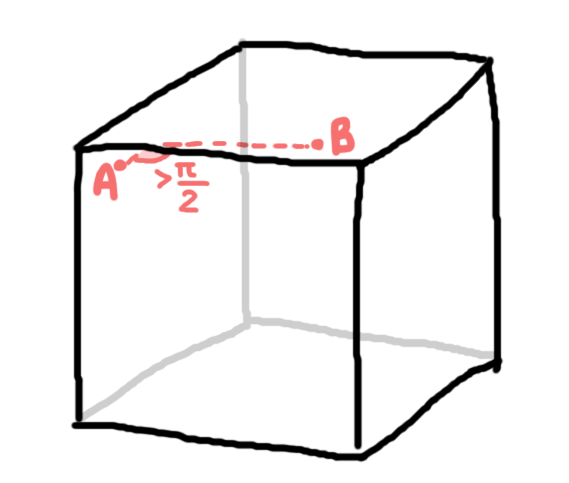
\includegraphics[width=0.3\linewidth]{contre_ex_0.png}
    \caption{Contre exemple pour la majoration de tout arc par $\frac{\pi}{2}$}.
    \label{fig:contre_ex_0}
\end{figure}

\textbf{intuition} : l'arc le plus court reliant deux points issues de faces adjacentes possède une courbure totale minimale.
$\rightarrow$ cela semble être encore faux (cf figure \ref{fig:contre_ex_1})...

\begin{figure}[!h]
    \centering
    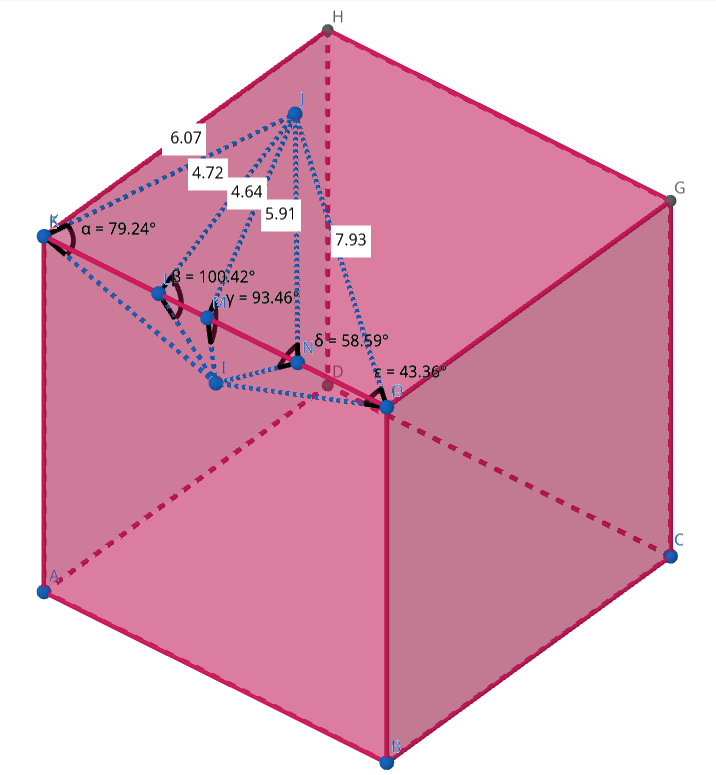
\includegraphics[width=0.5\linewidth]{contre_ex_1.png}
    \caption{Contre exemple pour la correlation entre la longueur de la ligne polygonale et sa courbure : la ligne polygonale JMI (troisième ligne) reliant les points J et I possède la plus petite longueur (4.64), mais sa courbure n'est pas minimale}
    \label{fig:contre_ex_1}
\end{figure}

\textbf{intuition} : la projection orthogonale du milieu du segment sur l'arête possède la plus petite courbure.\\
$\rightarrow$ Faux, voir contre exemple en figure \ref{fig:contre_ex_2}

\begin{figure}[!h]
    \centering
    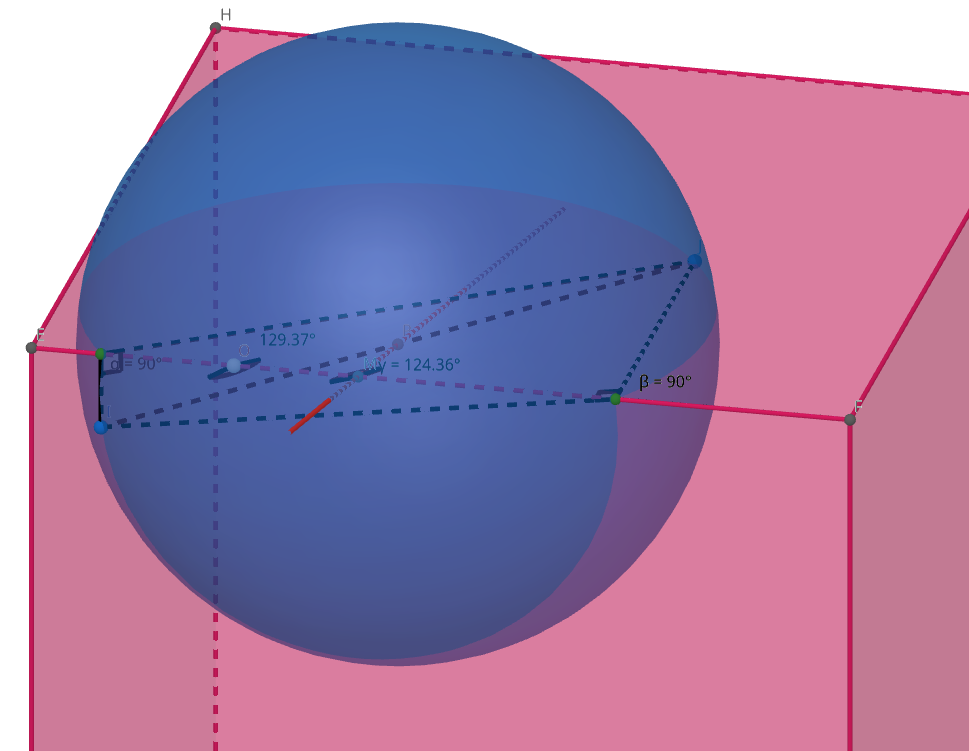
\includegraphics[width=0.5\linewidth]{contre_ex_2.png}
    \caption{Contre exemple pour la projection orthogonale du milieu du segment IJ : la projection est le deuxième point est possède un angle interne de 124.36° qui n'est pas maximal puisque le point 0 à sa gauche possède un angle de 129.37°.}
    \label{fig:contre_ex_2}
\end{figure}

\textbf{intuition} : la projection orthogonale du centre de la plus petite sphère passant par I et J et adjacent à l'arête forme un point K tel que l'angle IJK soit minimal (voir preuve).

\textbf{idées rejetées pour la preuve } :
\begin{itemize}
    \item En se plaçant dans un repère aligné sur le cube avec $A(0, y_A, z_A)$ et $B(x_B, 0, z_B)$, $O(x, y, z)$ et $C(0, 0, z)$, résoudre le système :
\begin{equation}
    \begin{cases}
      d(O, C) = d(A, O)\\
      d(O, C) = d(B, O)
    \end{cases}\,.
\end{equation}
Donne un $OC^2$ de degré 4 qu'il faut minimiser par rapport à $z$, ce qui est trop compliqué.
    \item En se plaçant dans le plan médiateur de $A$ et $B$ avec comme origine $I$ le milieu de $AB$, il n'est pas utile d'ajouter la contrainte de l'inclusion de $C$ dans le plan $AOB$ : cela signifierai que la famille de vecteurs $\overrightarrow{OA} = (-x_A, y_O, z_O)$, $\overrightarrow{OB} = (x_A, y_O, z_O)$ et $\overrightarrow{OC} = (- x_C, y_O - y_C, z_O - z_C)$ est liée, d'où :
    \begin{align*}
        &&                 \begin{vmatrix}
                          -x_A & x_A & -x_C\\
                           y_O  & y_O & y_O - y_C\\
                           z_O  & z_O & z_O - z_C
                           \end{vmatrix} &= 0\\
        \Leftrightarrow && -x_A \begin{vmatrix}y_O & y_O - y_C\\z_O & z_O - z_C\end{vmatrix} - x_A \begin{vmatrix}y_O & y_O - y_C\\z_O & z_O - z_C\end{vmatrix} + x_C \begin{vmatrix}y_O & y_O\\z_O & z_O\end{vmatrix} &= 0\\
        \Leftrightarrow && -2x_A(y_O(z_O - z_C) - z_O(y_O - y_C)) + x_C(y_Oz_O - z_Oy_O) &= 0\\
        \Leftrightarrow && -2x_A(y_O(z_O - z_C) - z_O(y_O - y_C)) &= 0\\
        \Leftrightarrow && -2x_A(y_Oz_O - y_Oz_C - z_Oy_O + z_Oy_C)) &= 0\\
        \Leftrightarrow && -2x_A(z_Oy_C - y_Oz_C)) &= 0\\
    \end{align*}
    Ainsi, on a $\boxed{z_Oy_C = y_Oz_C}$ or cette équation n'est pas utile à notre système.

    \item \textbf{Cercle circonscrit 1}

On sait que le point $C$ donne un angle maximal lorsqu'il correspond au projeté orthogonal du centre O du cercle circonscrit à A, C et B. 
En posant $A = (0, y_A, z_A)$, $B= (x_B, 0, z_B)$ et $C = (0, 0, z_C)$, on cherche $O(x, y, z_C)$ tel que $d(O, A) = d(O, C) = d(O, B)$ et $O$ est inclu dans le plan formé par $A$, $B$ et $C$ d'équation :
$$x(y_A)(z_B - z_C)) + y(x_B(z_A - z_C)) = 0$$
Cela revient donc à résoudre le système suivant :

\begin{equation}
    \begin{cases}
      x^2 + y^2 = x^2 + (y - y_A)^2 + (z_C - z_A)^2\\
      x^2 + y^2 = (x - x_B)^2 + y^2 + (z_C - z_B)^2\\
      x(y_A)(z_B - z_C) + y(x_B)(z_A - z_C) = 0
    \end{cases}\,.
\end{equation}

Les deux premières équations nous donnent :
$$x = \frac{(z_C - z_B)^2 + x_B^2}{2x_B} \text{ et } y = \frac{(z_C - z_A)^2 + y_A^2}{2y_A}$$

En substituant $x$ et $y$ dans la dernière équation, on résoud l'équation suivante pour trouver $z_C$ : 

\begin{align*}
\frac{((z_C - z_B)^2 + x_B^2)(y_A)(z_B - z_C)}{2x_B} + \frac{((z_C - z_A)^2 + y_A^2)(x_B)(z_A - z_C)}{2y_A} &= 0\\
((z_C - z_B)^2 + x_B^2)(2y_A^2)(z_B - z_C) + ((z_C - z_A)^2 + y_A^2)(2x_B^2)(z_A - z_C) &= 0\\
\end{align*}

\item \textbf{Cercle circonscrit 2}

On cherche $C$ tel que le cercle circonscrit à $A = (0, y_A, z_A)$, $B= (x_B, 0, z_B)$ et $C = (0, 0, z_C)$ soit de rayon minimal. 

Notons $a = d(A, B)$, $b = d(B, C)$ et $c = d(C, A)$.\\
On cherche à minimiser la fonction suivante :
$$R = \frac{abc}{4A}$$
Avec $A$ l'aire de $ABC$ défini par la formule de Héron comme $A = \sqrt{s(s - a)(s - b)(s - c)}$ où $s = \frac{a + b + c}{2}$.

On a $a = x_B^2 + y_A^2 + (z_A-z_B)^2$, $b = x_B^2 + (z_B-z)^2$, et $c = + y_A^2 + (z_A-z)^2$
\end{itemize}









\end{document} 